%% tikzlibraryforsyde.pictures.logo.code.tex
%% Copyright 2016-2018 George Ungureanu
%
% This work may be distributed and/or modified under the
% conditions of the LaTeX Project Public License, either version 1.3
% of this license or (at your option) any later version.
% The latest version of this license is in
%   http://www.latex-project.org/lppl.txt
% and version 1.3 or later is part of all distributions of LaTeX
% version 2005/12/01 or later.
%
% This work has the LPPL maintenance status `maintained'.
% 
% The Current Maintainer of this work is George Ungureanu.
%
% This work consists of the files listed in LICENSE.

\usetikzlibrary{calc}
\definecolor{KTHBlue}{RGB}{0,108,183}
\def\KTHBlue{KTHBlue}
\def\KTHDarkBlue{black!35!KTHBlue}
\def\KTHLightBlue{KTHBlue!25}

\newsavebox{\ForSyDeApplication}
\savebox{\ForSyDeApplication} {
  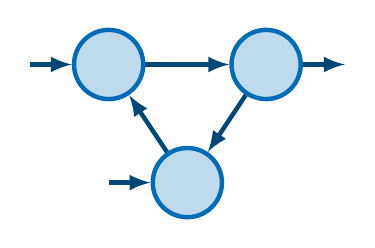
\begin{tikzpicture}
    [proc/.style={circle,draw=\KTHBlue,ultra thick,align=center,fill=\KTHLightBlue, minimum size=2.5em},
    ]
    \node[proc] (a) at (0,-0.5) {};
    \node[proc] (b) at (-1,1) {};
    \node[proc] (c) at (1,1) {};
    \path[-latex, ultra thick, \KTHDarkBlue] (a) edge (b) edge[latex-] (c) (b) edge (c)
    ($(b)-(1,0)$) edge (b) ($(a)-(1,0)$) edge (a) (c) edge ($(c)+(1,0)$);
  \end{tikzpicture}
}

\newsavebox{\ForSyDeImplementation}
\savebox{\ForSyDeImplementation}{

\begin{tikzpicture}[every path/.style={\KTHDarkBlue}]
  \draw [very thick, rounded corners=5pt] (0,0) -- (1,0) -- (1,1) -- (0,1) -- cycle;
  \foreach \i in {0,1,2,3,4} {
    \pgfmathsetmacro{\x}{.2 + \i * (.6 / 4) }
    \draw[very thick] (0,\x) -- (-.15,\x);
    \draw[very thick] (1,\x) -- (1.15,\x);
    \draw[very thick] (\x,0) -- (\x,-.15);
    \draw[very thick] (\x,1) -- (\x,1.15);
  }
  \node[circle, fill, draw, inner sep=.5pt] at (.2,.2) {};
  \node[circle, fill=white, very thick, draw, inner sep=7.5pt] (clock) at (.8,.2) {};
  \draw[very thick] ($(clock)+(0,7.5pt)$) -- (clock.center) -- ($(clock)+(5pt,0)$);
\end{tikzpicture}
}

\newsavebox{\ForSyDeLogo}
\savebox{\ForSyDeLogo} {

\begin{tikzpicture}[even odd rule]
  \def\ForSyDeLogoRadius{1.5}
  \def\ForSyDeLogoInnerRadius{1.3}
  \def\ForSyDeLogoJointAngle{30}
  \coordinate (left) at (0,0); 
  \coordinate (right) at (3.5,0);
  \def\binocularbackgroundcolor{\KTHDarkBlue} % was black!70
  \def\binocularcolor{\KTHBlue}
  
  % binocular background path
  \path[fill=\binocularbackgroundcolor]
  ([shift=(150:\ForSyDeLogoRadius)]left)
  to [bend left=17pt] ([shift=(85:1.3*\ForSyDeLogoRadius)]left)
  to [bend left=50pt] ([shift=(40:1.4*\ForSyDeLogoRadius)]left)
  to [bend left=18pt] ([shift=(-30:\ForSyDeLogoInnerRadius)]left)
  arc (-30:150:\ForSyDeLogoInnerRadius)
  ([shift=(30:\ForSyDeLogoRadius)]right)
  to [bend right=17pt] ([shift=(95:1.3*\ForSyDeLogoRadius)]right)
  to [bend right=50pt] ([shift=(140:1.4*\ForSyDeLogoRadius)]right)
  to [bend right=18pt] ([shift=(210:\ForSyDeLogoInnerRadius)]right)
  arc (210:30:\ForSyDeLogoInnerRadius)
  ;
  
  % goggles
  \path[fill=\binocularcolor] (left)  circle (\ForSyDeLogoRadius)  circle (\ForSyDeLogoInnerRadius);
  \path[fill=\binocularcolor] (right) circle (\ForSyDeLogoRadius)  circle (\ForSyDeLogoInnerRadius);

  % binocular joint path
  \path[fill=\binocularcolor]
  ([shift=(-\ForSyDeLogoJointAngle:\ForSyDeLogoRadius)]left) arc (-\ForSyDeLogoJointAngle:\ForSyDeLogoJointAngle:\ForSyDeLogoInnerRadius)
  to [bend right]
  ([shift=(180-\ForSyDeLogoJointAngle:\ForSyDeLogoInnerRadius)]right) arc (180-\ForSyDeLogoJointAngle:180+\ForSyDeLogoJointAngle:\ForSyDeLogoInnerRadius)
  to [bend right]
  ([shift=(-\ForSyDeLogoJointAngle:\ForSyDeLogoInnerRadius)]left);

  % elements.
  \node[scale=.55] at (left) {\usebox{\ForSyDeApplication}};
  \node[scale=1.2] at (right) {\usebox{\ForSyDeImplementation}};
\end{tikzpicture}
}